\chapter{Rozbor řešené problematiky}

TOTALNE PREKOPAT TENTO UVOD ROZBORU

Počítačový výkon je ůčinnost daného systému neboli jak dobře funguje, když se vezmou v úvahu všechny možné aspokty.
Hodnocení výkonu počítače je definováno jako proces při kterém se posuzují zdroje a výstupy počítače, aby se zjistilo,
jestli systém funguje na optimální úrovni.

Počítačové vyhodnocování je složitý proces. Při vyhodnoconváůní výkonu počítače se k určení využívá řada aspektů.
\paragraph{Hlavní aspekty}\cite{MetricsToday}
\begin{itemize}
    \item{škálovatelnost}
    \item{stabilita}
    \item{schopnost reagovat}
    \item{rychlost}
    \item{dostupnost}
    \item{propustnost}
    \item{doba odezvy}
    \item{spolehlivost}
    \item{provozuschopnost}
\end{itemize}

Napsat to do vysvetlivek a vysvetlit i zbytek, popsat jeste nejake metriky nize
Propustnost. Propustnost je počet jednotek dat, které systém zpracuje za určitou dobu.
Doba odezvy. doba odezvy měří, kolik času trvá systému, než zareaguje na dotaz nebo poptávku.
Spolehlivost, dostupnost a provozuschopnost (RAS). RAS označuje schopnost softwaru trvale plnit své specifikace; jak dlouho funguje vzhledem k očekávanému množství; a jak snadno se dá opravit nebo udržovat.

Ke zjištění těchto aspektů se využívají speciálně navržené programy, které posuzují relativní výkon daného objektu obvykle spušténím řady testů.
Tento proces se nazývá benchmark. Není jednoduché vytvořit měřítka pro hodnocení výkonu počítaču, protože technologické vlastnosti se stále vývýjí a obměňují.
Toto znamené, že benchmark počítačů musí být také neustále vyvíjen a aktualizován.

\iffalse
https://study.com/academy/lesson/computer-performance-evaluation-definition-challenges-parameters.html
\fi

\section*{Metriky k měření}

Před každým měřením by mělo být jasně dáno jaké metriky budeme měřit a jakým způsobem se to bude vykonávat. Pokud metriky ani způsob nebude stanoven, tak je měření ztrátou času.
Ověření těchto metrik se poté provádí testováním. Svoji důležitou roli hraje také složitost tesovaného softwaru. Mezi základní metriky k měření výkonu systému jsou:

\subsection*{Doba spuštění a doba načítání}

Každý software vyžaduje nějaký čas k jeho načtení a zahájení provozu. Koncový uživatelé během této doby obvykle vidí animovaný kurzor nebo načítání obrazovky.
Složité programy mohou vyžadovat nastavení a konfiguraci než uživatele pustí do práce. Software například kontroluje závislost s jiným softwarem nebo existenci potřebných souborů.
Toto zvyšuje jeho dobu načítání. Doba načítání by proto měla být co nejkratší.

\subsection*{Doba odezvy nebo latence}

Doba odezvy označováná jako latence je doba prodlevy mezi okamžikem, kdy uživatel zadá vstup, a okamžikem, kdy daný software na základě tohoto vstupu reaguje.
V ideálním připadě by tato doba měla být pro uživatele neposřehnutelná. Tato doba také může záviset na hardaru nebo na rychlosti připojení.

\subsection*{Omezené zatížení nebo špatná škálovatelnost}

Aplikace by měly obsluhovat omezený počet zařízení nebo uživatelů bez snížení výkonu softwaru. Škálovatelnost pomáhá zajistit, aby aplikace měla prostředky pro podporu očekávaného počtu uživatelů.
Testování výkonu hodnotí software při různých podmínkách zátěže. Nedostatečné zdroje, jako je nedostatečný výpočetní výkon, mohou způsobit špatnou škálovatelnost.
Výkon softwaru je však prostředky plus návrh a mnoho problémů se škálovatelností vyplývá ze špatné architektury aplikací. Každá aplikace by měla být napsaná tak, aby se dala v budoucnu škálovat.

\subsection*{Bottlenecks neboli uzká místa} napsat co to znamena v čestine

Každá aplikace přistupuje k omezenému zdrojů, jako třeba výpočetní výkon, paměťový prostor, šířka pásma, propustnost sítě, kapacita diskového ůložiště a vstupy/výstupy
a služby operačního systému. Úzká místa jsou nedostatky zdrojů, ke kterým dochází pokud software není vhodně navržen nebo pokud systém pro danou aplikaci není dostačující.

\iffalse
https://searchsoftwarequality.techtarget.com/answer/Required-prerequisites-for-performance-testing
\fi

\section{Metody}

Vyhodnocování výkonu počítačů je důležitou technologii pro výzkum v oblasti počítačů. Neustálý vývoj počítačů dělá tento úkol stále složitější.
Obecný problém rozvoje efektivní vyhodnocovací techniky lze vyjádřit jako hledání nejlepšího kompromisu mezi přesností a rychlostí. Tento kompromis závisí na
použití vyhodnocovací metody. Správná efektivita může vést ke snížení nákladů při tvorbě systému pro běh aplikace.

\section{Testování}

Vzhledem k velkému potenciálu hrozeb v souvislosti s výkonem softwaru, mohou různé testy zaměřené na výkon vyhodnitit specifické chování softwaru. Mezi důležité typy testů patří:
\begin{itemize}
    \item{zátěžový}
    \item{odolnostní}
    \item{spike}
    \item{závislostní}
\end{itemize}

\subsection*{Zátěžové testy}

Tento typ testů obecně měří pohyb dat, také nazývaný jako propustnost. Zátěživý test pomáhá ověřit zda daný software funguje správně za typických podmínek. Cílem zátěžového testování je zajistit,
aby klíčové metriky výkonu, jako propustnost dat za sekundu nebo přístup disku za sekundu, zůstaly přijatelné, když se připojí více zařízení nebo více uživatelů. Pokud testování významně
ovlivňuje metriky výkonu, tak je to signál k úpravě softwaru. Případně zjištění maximálního limitu softwaru.

\subsection*{Odolnostní testy}

Odolnostní testy jsou charakteristické tím, že se provádí po delčí dobu. Jejich cílem je ověřit, jestli se výkonnostní charakteristiky softwaru v průběhu provádění nemění. Odolnostní testy
zachycují nedostatky jako je nedostatečná paměť. Při krátkém testování by se tento problém nemusel vůbec objevit.

\subsection*{Spike testy}

Spike testy simulují náhle změny uživatelské zátěže za účelem měření odezvy softwaru.

\subsection*{Závislostní testy}

Software zřídka funguje sám o sobě. Většinou spoléha na jiné aplikace nebo případně na databázi. Testy závislosti vyhodnocují výkon softwaru při zátěži, ale vztahují se na závislosti, nikoliv
jen na software.

\iffalse
https://searchsoftwarequality.techtarget.com/answer/Required-prerequisites-for-performance-testing
\fi

\iffalse
\subsection{Existující řešení}
\fi

\section{Přehled nástrojů}

\subsection{Berkeley Packet Filter}

Berkeley Packet Filter nebo také BPF je technologie, která umožňuje spouštět programy v jádře operačního systému na linuxových systémech.
Efektivně a bezpečně rozšíří schopnosti jádra bez nutnosti měnit zdrojový kód jádra. Tato schopnost je často použita ke sledování využití systému či sledování síťového provozu.
BPF je k dispozici na většině unixových operačních systémů a extended BPF je také k dispozici pro Microsoft Windows.

\subsection*{Sledování síťového provozu}
BPF poskytuje rozhranní k datové lince, což umožňuje odesílání a přijímání paketů spojové vrstvy. BPF podporuje filtrování paketů a umožňuje user space(vysvětlit proč jsem to napsal anglicky) procesům,
aby si samy vyfiltrovaly pakety, které chtějí obdržet a které naopak zahodit. Toto může vést ke zvýšení výkonu operačního systému, protože se tím zamezí kopírování nepotřebných paketů.

\subsection*{Verze BPF}
BPF má více verzí. Výše zmíňenou extended BPF (eBPF) nebo také classic BPF (cBPF).

\subsection*{extended BPF - eBPF}
Extended BPF povoluje spouštět programy v rámci operačního systému a přidávat další funkce za běhu.
Operační systém pak zaručuje bezpečnost a efektivitu provádění. Díky to tomu je na eBPF je založeno hned několik projektů.
eBPF se používá pro  poskytování vysoce výkonných sítí a vyvažování zátěže v moderních datových centrech a cloudových nativních prostředích,
získávání podrobných dat o pozorovatelnosti zabezpečení při nízké režii, pomáhá vývojářům aplikací sledovat aplikace,
poskytování přehledů pro řešení problémů s výkonem a mnoho dalšího.

\subsection*{classic BPF - cBPF}
Classic BPF je jenom přejmenovaná originální verze BPF.

\iffalse
https://man7.org/linux/man-pages/man2/bpf.2.html
https://ebpf.io/
\fi

\subsection{Netem}
Netem\cite{Netem} je softwarová utilita pomocí které lze vykonávat síťovou emulaci. Síťovou emulaci lze využít k omezení internetových zdrojů pro měřenou aplikaci pro lepší testování.
Netem umí simulovat zpomalení, ztrátu, poškození nebo duplikaci paketů a případně změnu pořadí paketů. Netem je řízen pomocí nástroje 'tc', který se ovládá pomocí příkazové řádky.
Jeho aktuální distribuce je multiplatformě podporována.

\subsection*{Zpoždění paketů}
Tento příkaz přidá zpoždění všech paketů o 100 milisekund. Toto nastavení je ještě omezeno rozlišením jádra.
\begin{lstlisting}[language=bash]
    $ tc qdisc add dev <interface> root netem delay 100ms
\end{lstlisting}

Lze i nastavit zpoždění pomocí rozdělení. Příklad s normalním rozdělením:
\begin{lstlisting}[language=bash]
    $ tc qdisc change dev <interface> root netem delay 100ms 20ms distribution normal
\end{lstlisting}

\subsection*{Ztráta paketů}
Tento příkaz zajistí ztrátu paketů. 1 paket z 1000 je zahozen. Nejnižší možná nastavitelná hodnota je 0.0000000232%.
\begin{lstlisting}[language=bash]
    $ tc qdisc change dev <interface> root netem loss 0.1%
\end{lstlisting}

\subsection*{Duplikace paketů}
Příkaz pro duplikaci paketů je podobný jako příkaz pro ztrátu paketů.
\begin{lstlisting}[language=bash]
    $ tc qdisc change dev <interface> root netem duplicate 1%
\end{lstlisting}

\subsection*{Poškození paketů}
Tímto příkazem lze nastavit poškození paketů. Ten zavede bitovou chybu v náhodném offsetu v paketu.
\begin{lstlisting}[language=bash]
    $ tc qdisc change dev <interface> root netem corrupt 0.1%
\end{lstlisting}

\subsection*{Přeuspořádání paketů}
Existují dva způsoby jak nastavit přeuřpořádání paketů.
První způsob je pomocí metody gap, která používá přednastavenou sequekci a změní pořadí každého Ntýho paketu.
\begin{lstlisting}[language=bash]
    $ tc qdisc change dev <interface> root netem gap 5 delay 10ms
\end{lstlisting}
Druhá metoda je reorder způsobí, že určité procento paketů se špatně seřadí.
\begin{lstlisting}[language=bash]
    $ tc qdisc change dev <interface> root netem delay 10ms reorder 25% 50%
\end{lstlisting}

\subsection*{Obnovení rozhranní}
Tento příkaz smaže všechno nastavení na rozhranní. Rozhranní bude poté fungovat jako by na něm žádné nastavení nebylo.
\begin{lstlisting}[language=bash]
    sudo tc qdisc del dev <interface> root
\end{lstlisting}


Mozna pridat do testovani a ne tady

testovano na debian, ubuntu, Raspberry

\subsection{Virtuální počítač s omezenými zdroji}

Pro zajištění více testovacích platforem je jedna z
Bohužel výpočetní hardware bude stejný pro všechny virtuální platformy i když bude omezený.

\iffalse
\subsection*{Raspberry pi}
github.com/raspberrypi
\fi



\chapter{Fungování operačního systému linux}

Aby bylo možné s operačním systémem linux pracovat je potřeba vědět jak vlastně celý systém funguje. Při tvorbě běžných aplikací není potřeba
znát operační systém linux nějak dokonale. Ovšem pokud aplikace pracuje v prostoru jádra(PRIDAT ODKAZ), je nutností vědět jak linuxový operační
systém funguje a poté vyhodnotit zda aplikace nemůže nějakým způsobem poškodit tento systém. Aplikace, které jakkoliv pracují v prostou
jádra musí být spuštěny s příkazem sudo(ODKAZ) jako super uživatel. Tímto způsobem aplikace získá možnost pracovat v prostoru jádra bez
omezení.

\section{Vrsty linuxového systému}

Linuxový systém se skládá ze 3 úrovní, které můžeme vidět na obrázku níže.(ODKAZ na obrazek)
Jak je již zmíněno výše, tak aplikace mohou pracovat v uživatelském prostoru nebo v prostoru jádra.

\begin{figure}
    \centering
    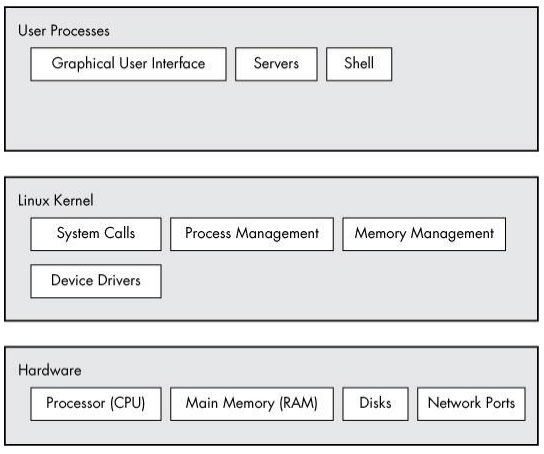
\includegraphics{obrazky-figures/linux_structure.png}
    \caption{}
    \label{}
\end{figure}

\subsection{Hardware}
Hardware je základ každé výpočetní jednotky. Skládá se z paměti, procesor, disku a síťového rozhranní. Tato úroveň je nejnižší z těchto tří
úroveňí.

\subsection{Linuxové jádro}
Další úrovní je linuxové jádro, což je také jádro operačního systému. Jádro je umístěné v paměti, která se také nayývá prostor jádra
(angl. kernel space). Je zde uložen a vykonávám kód jádra, který taktéž řídí procesor a říká mu co má dělat.
Jádro především funguje jako rozhranní mezi hardwarem a jakýkoliv spuštěným programem. Zároveň také jádro spravuje hardware.

\subsection{Uživatelské procesy}
Běžící programy, které jádro spravuje, tvoří nejvyšší úroveň systému. Je také nazýván jako uživatelský prostor.
Uživatelský prostor(angl. user space) je sada míst, kde běží uživatelské procesy(všechno ostatní kromě jádra). Jádro řídí aplikace v tomto
prostoru tak, aby se nepletly mezi sebou. Procesy, které běží v uživatelském prostoru mají omezenou část paměti a také nemají přístup do
prostoru jádra. Procesy běžící v uživatelském prostoru mohou přistupovat do prostoru jádra jedině přes rozhranní vystavenné prostorem
jádra - systémová volání(ODKAZ NA SYSTEMOVA VOLANI). Pokud proces provede systémové volání, tak se do jádra odešle systémové přerušení
a jádro poté obslouží příslušný proces. Jádro pokračuje ve své práci až po dokončení přerušení.

\subsection*{Rozdíly}
Kód běžící v prostoru jádra má neomezený přístup k hlavní paměti a procesoru. Toto je velice silné, ale zároveň velmi nebezpečné privilegium.
Procesy, které zde běží, mohou snadno havarovat celý systém a tím ho nenávratně poškodit.

Naopak v uživatelském prostoru je přístup do paměti omezený na malou podmnožinu a bezpečné operace v procesoru. Jestliže proces z nějakého
důvodu udělá chybu a havaruje, tak jeho následky jsou omezené a jádro je může vyčistit.

Ovšem proces v uživatelském prostoru může také způsobit poškození. Když bude mít vyšší oprávnění než jiné procesy, tak může třeba přepsat
data uložená na disku. Proto je i toto potřeba, dávat si pozor.

\iffalse
www.linfo.org/kernel_space.html
kniha How linux works
\fi

\subsection{Datové struktury}
ringbuffer = popsat, slozitost
popsat i ostatni datove struktury

\subsection{Sledovací bod}
Sledovací bod(angl. tracepoint) umístěný ve zdrojovém kódu poskytuje tzv. háček pro volání funkce(sondy) poskytnutou za běhu aplikace.
Sledovací bod může být zapnutý, pokud je k němu připojena nějaká sonda nebo vypnutý, jestliže k němu žádná sonda připojená není. Když je
sledovací bod zapnutý, tak volá poskytnutou funkci, pokaždé když je sledovací bod spustěň v kontextu provádění volajícího. Když poskytnutá
funkce ukončí své provádění, tak se vrací k volajícímu(pokračuje z místa sledovacího bodu).

Lze je využít pro sledování sýstému nebo výkonu.

\iffalse
https://www.kernel.org/doc/Documentation/trace/tracepoints.rst
\fi

\subsection {Sledování událostí}
Sledovací body lze využít ke připojení funkce k určité události.

\subsection*{Formát}
Každý trasovatelná událost má soubor "format", který obsahuje popis každého pole daného eventu. Tyto informace lze poté využít v další
analýze. Dále také zobrazuje formátovací řetězec pro tisk události v textovém režimu, název události a ID pro profilování.

Pole v souboru "format" má tvar:
field:field-type field-name; offset:N;velikost:N;
Offset je posun pole v záznamu trasování a velikost je velikost dané datové položky určená v bajtech.

Jako příklad je uvedena událost(systémové volání) openat:

\begin{verbatim}
name: sys_enter_openat
ID: 623
format:
	field:unsigned short common_type;	offset:0;	size:2;	signed:0;
	field:unsigned char common_flags;	offset:2;	size:1;	signed:0;
	field:unsigned char common_preempt_count;	offset:3;	size:1;signed:0;
	field:int common_pid;	offset:4;	size:4;	signed:1;

	field:int __syscall_nr;	offset:8;	size:4;	signed:1;
	field:int dfd;	offset:16;	size:8;	signed:0;
	field:const char * filename;	offset:24;	size:8;	signed:0;
	field:int flags;	offset:32;	size:8;	signed:0;
	field:umode_t mode;	offset:40;	size:8;	signed:0;

print fmt: "dfd: 0x%08lx, filename: 0x%08lx, flags: 0x%08lx, mode: 0x%08lx", ((unsigned long)(REC->dfd)), ((unsigned long)(REC->filename)), ((unsigned long)(REC->flags)), ((unsigned long)(REC->mode))
\end{verbatim}

\iffalse
https://www.kernel.org/doc/Documentation/trace/events.rst
\fi

\subsection{Systémové volání}

V moderních operačních systémech poskytuje jádro sadu rozhranní pomocí kterého procesy běžící v uživatelském prostoru můžou interagovat
se systémem. Tato rozhranní poskytují aplikacím přístup k hardwaru, což je mechanismus, díky kterému se dají vytvářet nové procesy,
komunikova se stávájícími a výžádat si operační systém o další zdroje. Existence těchto rozhranní a faktem, že aplikace si nemohou přímo
dělat, co chtějí, je klíč ke stabilnímu systému.

Systémové volání\cite{LinuxKernelDevelopment} jsou typicky přístupné přes funkce v C knihovně a mají předem definované chování. Mají nula
a více argumentů a můžou mít i návratové hodnoty. Obvykle v typu long. Nula je většinou značení pro uspěch a záporná hodnota značí chybu.
Pokud systémové volání vrátí chybu, tak vloží speciální chybnou hodnoru do globalní proměné zvané \emph{errno}. Hodnotu lze přeložit do
lidsky čitelné podoby pomocí funkce \emph{perror()}. Každé systémové volání má konvenci pojmenování, že začíná s \emph{sys_}.

\subsection*{Komunikace s kernelem}




POPSAT sudo = superuser